\chapter{Introduction}
\section{A little motivation}

The desire to infer precise and accurate stellar ages is motivated by a range
of scientific drivers, but the one that most sparks my personal interest is
the implications for understanding the evolution of exoplanetary systems.
Despite the rapidly accelerating interest in exoplanet population studies
\citep[e.g.][]{petigura, dressing, foreman-mackey, burke}, we still know very
little about how planetary systems {\it evolve}.
This is because stellar ages are difficult to infer.
{\bf I propose to develop a new dating method that will provide the most
precise and accurate stellar ages ever measured for hundreds of thousands of
stars, in order to study the evolution of exoplanetary systems.}

Planetary system architectures are not static in time: chaotic gravitational
interactions fling planets into interstellar space, plunge them into the
surface of their star, collide them together and excite them to highly
eccentric and inclined orbits.
Simulations show that planet losses are most common in the few millions of
years immediately after formation and continue at a gradually decreasing rate
\citep[e.g.][]{zhou, smith, funk, Pu2015}.
Planet-planet scattering on extended timescales will result in a {\it
detectable}\/decrease in exoplanet frequency with stellar host age in the
enormous sample of over five thousand planets discovered by the \Kepler\
spacecraft, as well as the complementary systems detected by the \Ktwo\ and
\TESS\ transit surveys, if their ages can be sufficiently constrained
\citep{veras}.
As I explain in this thesis, my research has advanced our understanding of the
stellar age-rotation, or `gyrochronology' relations \citep{angus}, which will
contribute to our ability to infer stellar ages with unprecedented precision
and, for the first time, search for variations in the architecture and
frequency of exoplanets as a function of host star age.

Studying the exoplanet population as a function of age will unveil the
processes behind planet formation and dynamical evolution---two extremely
active areas of research.
By evaluating planet occurrence rates over a range of stellar ages it will be
possible to examine the dependence of overall occurrence on age and constrain
the rate of exoplanet loss.
Once the loss-rate is known we can extrapolate back in time to reveal what
zero-age planetary systems look like.
By measuring the overall exoplanet loss-rate we can constrain the primordial
number of planets per star.

Stellar ages also provide a window into the {\it architectural}\/evolution of
planetary systems.
The exoplanet population shows a mysterious feature: half of all transiting
exoplanet systems have just one transiting planet and the other half have
multiple \citep[e.g.][]{lissauer, johansen, ballard}.
Additionally, the single planet systems, or `singles', are more often
misaligned with the spin-axis of their host star and have more eccentric
orbits than multiple planet systems, `multis' \citep[e.g.][]{morton, winn}.
This phenomenon is known as the `\Kepler\ dichotomy', and its origin is
a point of hot dispute: do two modes of formation create the distinct system
architecture?
\citet{Pu2015} propose an elegant solution: the singles are descended from the
multis, i.e.\ they are the remains of once ordered planetary systems, ripped
apart by chaotic gravitational interactions.
If this is the case, the singles may, on average, be older than the multis.
Most compact \Kepler\ multis are so tightly packed that they hover near the
stability limit \citep{fang}.
As the lifetime of a planetary system increases, so does its disruption
probability, therefore tightly-packed multis have shorter projected lifetimes
than loosely-packed systems.
By comparing the ages of tightly packed multis with the ages of loosely-packed
multis and the ages of singles it may be possible to reveal the dynamical
origins of the three groups.

The dominant mechanism for hot Jupiter migration is hotly debated and it is
unclear whether disc migration or orbital perturbation via gravitational
interaction is responsible for the majority of cases.
Distant stellar or planetary companions can excite planets onto orbits that
alternate between high eccentricities and high inclinations (known as
Kozai-Lidov, KL, oscillations).
Extremely small separations between the planet and host at periapsis during
the resulting periods of high eccentricity induce tidal forces that lead to
eventual orbital circularisation.
The timescales for excitation, followed by tidal circularisation are long,
therefore hot Jupiters produced via KL oscillations should be relatively old
\citep{petrovich}.
By inferring the ages of hot Jupiter hosts in may be possible to study the
frequency of KL oscillation-induced migration.

Exoplanet population studies are just one area of research that benefits from
stellar ages.
Another popular topic is galactic archaeology: the study of the formation
history of the Milky Way.

\section{The challenge of stellar age inference}

Ages are notoriously difficult to infer because stars vary little in brightness
or temperature during their hydrogen-burning lifetimes and fitting stellar
evolution models to these two observables usually produces age estimates with
uncertainties in the order of 50-150\%.
Fortunately, recently obtained asteroseismic ages and cluster star
observations will allow me, via a new hierarchical, probabilistic model,
to obtain an age measurement for every star observed by the \kepler,
\Ktwo\ and \TESS\ missions.

Because cool stars spin down predictably over their main sequence lifetime
due to magnetic braking, their ages depend, to first order, only on
their masses and current rotation periods \citep[e.g.][]{skumanich, kawaler,
barnes}, as shown in figure \ref{fig:gyro}.
Photometric measurements of these two parameters can therefore be used to
infer an age.
This is the unique selling point of gyrochronology---ages can be inferred from
photometry alone.
Earlier this year I used \Kepler\ asteroseismic field stars to calibrate
the gyrochronology relations at late ages, revealing a surprising result: the
old targets rotated more rapidly than expected \citep{angus}.
This finding provoked the response of \citet{vansaders} who attribute this
behaviour to an evolving magnetic dynamo.
Their result is important as it informs us over which range of stellar ages
the gyrochronology method delivers precise results.
Gyrochronology performs best for stars that are Solar-mass or below and/or
those that are younger than the Sun.
These criteria are met by most of the \Kepler\ stars: the age distribution
peaks at around 2 Gyr and the mass distribution is centered on Solar-mass
\citep{walk, mcquillan2014}.
For many of these stars gyrochronology can yield stellar ages with 20\%
precision \citep{epstein} and as demostrated by \citet{veras},
a time-resolution of 20\% is more than sufficient to detect variations in the
exoplanet occurrence rate over time.

Determining the detectability of trends in the ages of \Kepler\ systems is
challenging as the outcomes of simulations depend strongly on input
assumptions and different studies therefore produce different predictions
\citep[see figure 3 of][]{Pu2015}.
However, based on the \citet{smith} simulations of systems with three
Earth-mass planets, \citet{veras} demonstrate that a decrease in planet
occurrence rate will be detectable for K dwarf hosts, even if stellar age
uncertainties are as large as 5 Gyr, and for G dwarfs with age uncertainties of
3.5 Gyr.
Most systems do not consist of equal-mass planets, however their study
demonstrates that an age trend lies well within the realms of detectability.
Age precision will vary on a star-by-star basis, most likely ranging from
0.5-5 Gyr, however I expect to infer ages with uncertainties of $\sim$1 Gyr
for the majority of planet hosts and, thanks to the size of the Kepler planet
candidate sample, this will be more than sufficient to reveal trends in the
data.

\section{Stellar dating methods}

The hydrogen-burning era of a star's life is extremely stable.
This fact is unfortunate from a stellar chronologist's point of view: without
an observable property that is a strong function of age, stellar age precision
will always be limited.
This is the fundamental stopping-point for stellar age inference: age
precision is limited by the fundamental evolutionary time-scale of stars.
Despite this limitation however, there is still progress to be made in
understanding the evolution of the observable properties from both empirical
and theoretical standpoints, and in the precision with which we can measure
these properties.
In the following section I will describe some of the available dating methods,
their observational inputs and their limitations.

\subsection{Isochrone fitting}
As stars burn hydrogen they become hotter and more luminous and slowly move
towards the top right of the Hertzprung-Russel, or Colour-Magnitude Diagram
(CMD).
The variation in luminosity and temperature over time has been modelled by
several teams of astronomers, producing their own sets of model grids.
For example, the Dartmouth \citep{dotter}, Yonsei-Yale \citep{spada} models
are two of the most commonly used sets of models.
It is therefore possible to estimate the age of a MS star by fitting such
models to its luminosity and effective temperature or its colour and V-band
magnitude.
A limitation of this method however, is that the composition of the star in
question will affect its placement on the CMD and must therefore be known
precisely to yield a precise age.
This is often impossible since expensive, high-precision spectroscopy is
required to obtain the metallicity, helium abundance and alpha-element
fraction of a star.
However, for an ensemble of coeval stars with identical compositions this
process becomes much easier: not only are there more opportunities to measure
stellar compositions, providing a $\sqrt N$ reduction in measurement
uncertainty, a group stars with the same age and composition but different
masses will reveal the shape of the best-fitting isochrone on the CMD\@.
This reduces the need for knowing composition precisely in the first place.
For these reasons, many open stellar clusters have very precise ages.

% For example Pleiades (0.55 Gyr), Hyades (0.625 Gyr), Praesepe (0.588 Gyr), and
% Coma Berenices (0.5 Gyr).
% Download isochrones and estimate the ages of some KOIs.

\subsection{Asteroseismology}

Asteroseismology is a powerful dating method with the potential to yield
extremely precise stellar ages.
However, the era of asteroseismology has only just arrived and this fledgling
field is still only applicable to a small number of extremely bright stars
observed by precise photometric space-missions.

Oscillations in the Sun are caused by turbulent convection near the surface.
The movement of ionized gas stochastically excites the Sun's spherical
oscillation modes.
An analogy to this process is that of a bell in a room filled with air.
Air particles colliding with the surface of the bell cause it to vibrate at
all of its spherical harmonic frequencies.
There is no coherent driving force, rather the stochastic collisions of air
particles induce a continual ringing.
Similarly, the Sun is continually oscillating at a range of discrete
frequencies; those that correspond to its spherical harmonics.
A power spectrum of the Sun, taken from \citet{brown} is shown in figure
~\ref{solar_spectrum}.
The comb-like, evenly spaced peaks in this power spectrum show Solar p-mode
oscillations.
The peak amplitudes are modulated by a Gaussian envelope.
The mean of that Gaussian, $\nu_{max}$ corresponds to a frequency of around
3000 \uHz, a period of around five minutes.

\begin{figure}[p]
\begin{center}
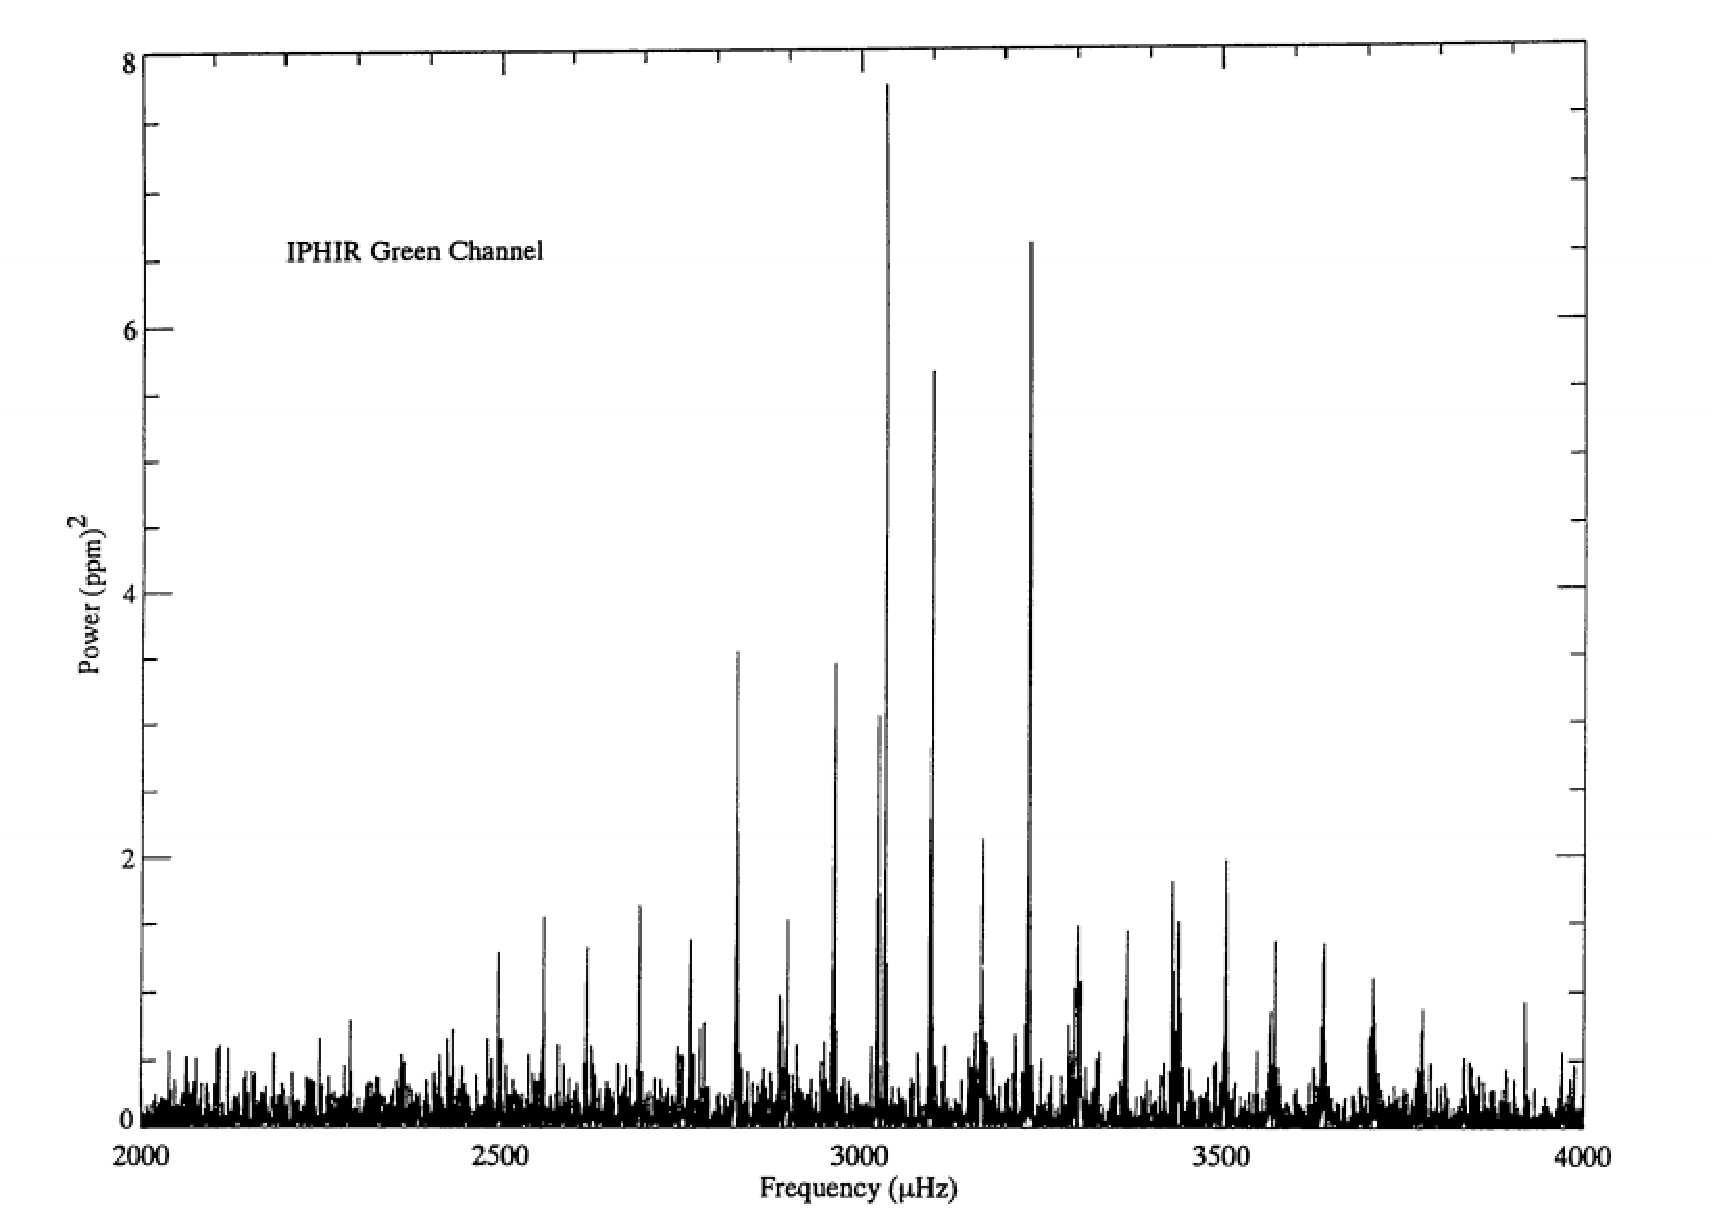
\includegraphics[width=6in, clip=true]{figures/solar_spectrum.pdf}
\caption{A power spectrum of one month of disk-integrated Solar photometry,
taken from \citet{toutain}. Solar p-modes are clearly visible in this figure.}
\label{fig:solar_spectrum}
\end{center}
\end{figure}

Many properties of the Sun have been measured using asteroseismic pulsations.
For example, the variation in radial pressure, the rate of differential
rotation, the depth and fraction of helium in its convective zone and even the
structure of active regions below the Solar surface.
The Sun is an exquisite example of a pulsating star, having tens of millions
of detectable modes and mode lifetimes that are several thousand times longer
than the periods of the oscillations.
Its proximity, which both provides enormous signal-to-noise and allows us to
resolve the surface, make it a paragon of seismology.

Three types of oscillations are detectable in the Sun: pressure, or p-modes,
surface, s-modes and gravity, g-modes.
Pressure provides the restoring force for p-mode oscillations, and these are
effectively sound waves.
Surface modes are, as the name suggests, waves on the surface of the star.
% Since it is only possible to detect s-mode waves if the stellar surface is
% resolvable, this type of wave has only been seen in our Sun.
G-modes are excited by buoyant gas in the radiative zone and the restoring
force is gravity, hence the name.
These waves rapidly evanesce in stellar convective zones and therefore
appear at very low amplitudes at the surface of Sun-like stars.
For the work in this thesis I am concerned only with p-mode observations, as
these waves reveal the internal structure of a star which varies as a function
of mass, radius and age.

The frequency of a p-mode wave is proportional to the sound-speed of the gas
along its path through the stellar interior.
Time-dependent spatial perturbations to a star's equilibrium state can be
written as a product of a term that depends on stellar radius and a spherical
harmonic (assuming that a star can be approximated as a sphere) as follows
\citep{brown},
\begin{equation}
    \xi_{nlm}(r, \theta, \phi, t) = \xi_{nl}(r)Y_l^m(\theta, \
    \phi)e^{-i\omega_{nlm}t}.
\end{equation}
$\xi$ is a spatial perturbation, associated with a mode, $r, \theta, \phi,
\omega$ and $t$ are the radial coordinate, colatitude, longitude angular
frequency\footnote{The convention in asteroseismology is to report circular
frequencies, $\nu_{nlm} = \omega_{nlm}/2$.} and time, respectively.
$n$ is the radial order, defined as the number of nodes between the star's
centre and surface and $l$ is the angular degree, the product of the stellar
radius and the total horizontal wavenumber of the mode.
For example, a star oscillating with an $l = 10$ mode will have a standing
wave with 10 nodes along a line around the equator.
Finally, $m$ is the azimuthal order; the projection of $l$ onto the horizontal
wavenumber of mode and must be less than or equal to $l$.
A star with an $m = 5$ mode will have a standing wave with 5 nodes along a
line connecting its poles.
The relation between $\omega$ and $n$ and $l$ is complicated and depends on the
structure of the star.
Oscillations with different values of $l$ penetrate to different depths in the
star.
$l = 0$ waves travel through the centre and waves with increasing $l$ skirt
the central region by a larger and larger distance.
For this reason, modes with different $l$ provide information about the sound
speed gradient in the stellar interior.
The `small frequency separation', $\delta_{n,l} = \nu_{n+1, l} - \nu_{n, l+2}$
is often used to parameterise the variation in frequency with stellar radius
via \citep{brown}
\begin{equation}
    \delta_{n,l} = \Delta\nu_0\frac{(l + 1)}{2\pi^2\nu_{nl}}\int_0^{R_\star}
    \frac{dc}{dr}\frac{dr}{r}.
\end{equation}
Since nuclear-burning material in the core changes its molecular weight as the
star evolves, the sound-speed gradient is time-dependent and the small
separation therefore contains information about the age of the star.

There is no simple harmonic relation between the frequencies of modes with
adjacent mode number \citep{brown}.
% check this!
However, in the limit where $n \gg l$, mode frequency can be approximated as
\begin{equation}
    \nu_{nl} = \Delta\nu_0\left(n + \frac{l}{2} + \epsilon \right) - \
    \frac{AL^2 - \eta}{(n + l/2 + \eta)},
\end{equation}
where parameters $\Delta\nu_0$, $A$, $\epsilon$ and $\eta$ depend on the
structure of the star and $L^2 = l(l+1)$.
$\Delta\nu_0$ is the `large frequency separation' which, together with the
peak frequency of the Gaussian envelope that modulates the amplitudes of the
oscillation modes, $\nu_{max}$, makes up the two fundamental asteroseismic
observables.
It is related to the sound travel time through the centre of the star:
\begin{equation}
\Delta\nu_0 = \left(2\int_0^{R_\star}\frac{dr}{c}\right)^{-1},
\end{equation}
where $c$ is the local sound speed and $R_\star$ is the stellar radius.
This travel time is related to the mean density of the star via,
\begin{equation}
\Delta\nu_0 \cong 135\left(\frac{M_\star}{R_\star^3}\right)^{1/2}\mu Hz,
\end{equation}
where $M_\star$ and $R_\star$ are the stellar mass and radius in Solar units
\citep{cox, brown}.

Today, p-modes have been detected in hundreds of Sun-like stars, however it
was not until the late 1990s that the first conclusive detection was made in
a star other than our Sun.
The reason for this is simply that p-mode perturbations are extremely
small---these changes are around 10 cms$^{-1}$ in velocity and 3$\mu$mag in
brightness for typical oscillation modes in the Sun \citep{brown2000}.
Asteroseismic pulsations are usually detected in two different ways: by
searching for the subtle change in luminosity caused by the temperature
fluctuations of the stellar surface, or by measuring the changing radial
velocity of the surface.
A Fourier transform of these time series will reveal the presence of
oscillation modes, allowing for the modelling of the star's interior
structure.
The earliest p-modes detections were made using radial velocity data
\citep{kjeldsen2001} for stars $\eta$ {\bf Boo} \citep{kjeldsen1995}, {\bf
Procyon} \citep{barban1999, martic1999}, $\zeta$ {\bf Herculis}
\citep{martic2001}, $\alpha$ {\bf Cen A} \citep{kjeldsen1999} and $\beta$ {\bf
Hyi} \citep{bedding2001}.
Today, we have the advantage of space-based missions \kepler and \corot whose
photometric precision provides sufficient signal-to-noise to detect
p-mode-induced luminosity variations.
These missions have provided fundamental parameters for hundreds of
oscillating giants, subgiants and Sun-like stars \citep[e.g.][]{michel2008,
bruntt2009, chaplin2014}.

% Extracting fundamental parameters from time series.
\subsubsection{Fundamental parameters from photometric time series}

In the previous section I describe the relations between stellar p-mode
oscillation frequencies and the physical parameters of a star.
In this section I will describe the application of asteroseismology: how
exactly does one infer fundamental stellar parameters from a light curve?
My thesis work focuses on \kepler data, so this discussion will be directly
related to \kepler data, but the same principles apply to other photometric
time series.

The \kepler spacecraft is a precise photometric space-telescope with two
differing but related primary objectives.
The original mission, often referred to as \kepler prime, pointed at a single
patch of sky, in the constellation of Lyra for four years almost continually
in order to search for transiting exoplanets.
Its primary objective was to allow us to infer the occurrence rate of
Earth-like planets.
The \kepler field was selected as a part of the sky that was not too crowded,
as a field in the galactic plane would be, yet containing enough stars that a
statistical sample of exoplanets could be accumulated.
The chosen field had around 150,000 stars that fell on silicon and were
downloaded from the spacecraft.
During the primary mission of \kepler, thousands of planet candidates were
discovered, of which over a thousand were subsequently either followed up with
radial velocity observations or confirmed dynamically by some other method.
\kepler prime's success story is not limited to exoplanets, however: stellar
astronomy itself has been advanced and arguably the second most important
branch of \kepler prime's legacy is asteroseismology.

\kepler operates in two observing modes: long and short cadence
\citep[][]{smith2012, stumpe2012}.
Long cadence observations are taken every approximately 30 minutes, with ...
minute integration times and short cadence observations are taken every minute
with ... second integration times.
The frequencies that are accessible to \kepler are limited by two things: the
duration of observations and the time sampling.
The duration of observations, e.g. the length of the \kepler mission sets the
minimum resolvable frequency.

This branch of astronomy is still relatively young and, given the quantity of
up-and-coming photometric space missions, will continue to provide precise
stellar parameters for decades to come.
However, accurate and precise asteroseismic ages demand high-precision
photometry of bright (brighter than around 12th magnitude) stars.
Even with \kepler and \corot, this only amounts to around one hundred MS
stars.
It is therefore essential that alternative dating methods, which can be
applicable to a much larger sample of stars are developed.
Age-rotation relations, for example.

Asteroseismology is the way forward for fundamental stellar parameters.
It provides precise and accurate parameters, against which models for age,
mass and radius can be calibrated.

\subsection{Age-activity and age-rotation relations}

Asteroseismology is revolutionising stellar astronomy and, perhaps, stellar
ages in particular (partly because the bar is so low to begin with).
However, it is not yet ready to  revolutionise fields involving stellar
populations because it is still a `boutique' method, applied to hand-picked,
bright, text-book Solar-like oscillators.
In order to produce a catalogue of stellar ages that is large enough to be
useful for studies of stellar populations, we need a method that can be
applied to thousands of stars \ie requires inexpensive observables, is not
computationally expensive and doesn't require human input (can be automated).
For this reason gyrochronology, the method of inferring an age from a rotation
period is an intriguing prospect as, if demonstrably accurate, fulfills all
the above criteria.

A decreasing trend in rotation period with age was first noticed in the
\citet{skumanich1972}.
In figure \ref{fig:skumanich}, equatorial rotational velocity vs time
(triangles) is plotted on the same axes as lithium abundance (crosses) and
Ca$^+$ emission (circles) for the Hyades and Pleiades clusters, as well as the
Sun.
The Sun is the far right point for each age indicator.
Only the equatorial velocities of the G stars in the two clusters are
indicated.
Ursa Major stars are included on the Ca$^+$ emission scale.
Lithium abundance and Ca$^+$ emission were previously known age indicators and
this work demonstrated the potential of rotation period as another.

\begin{figure}
\begin{center}
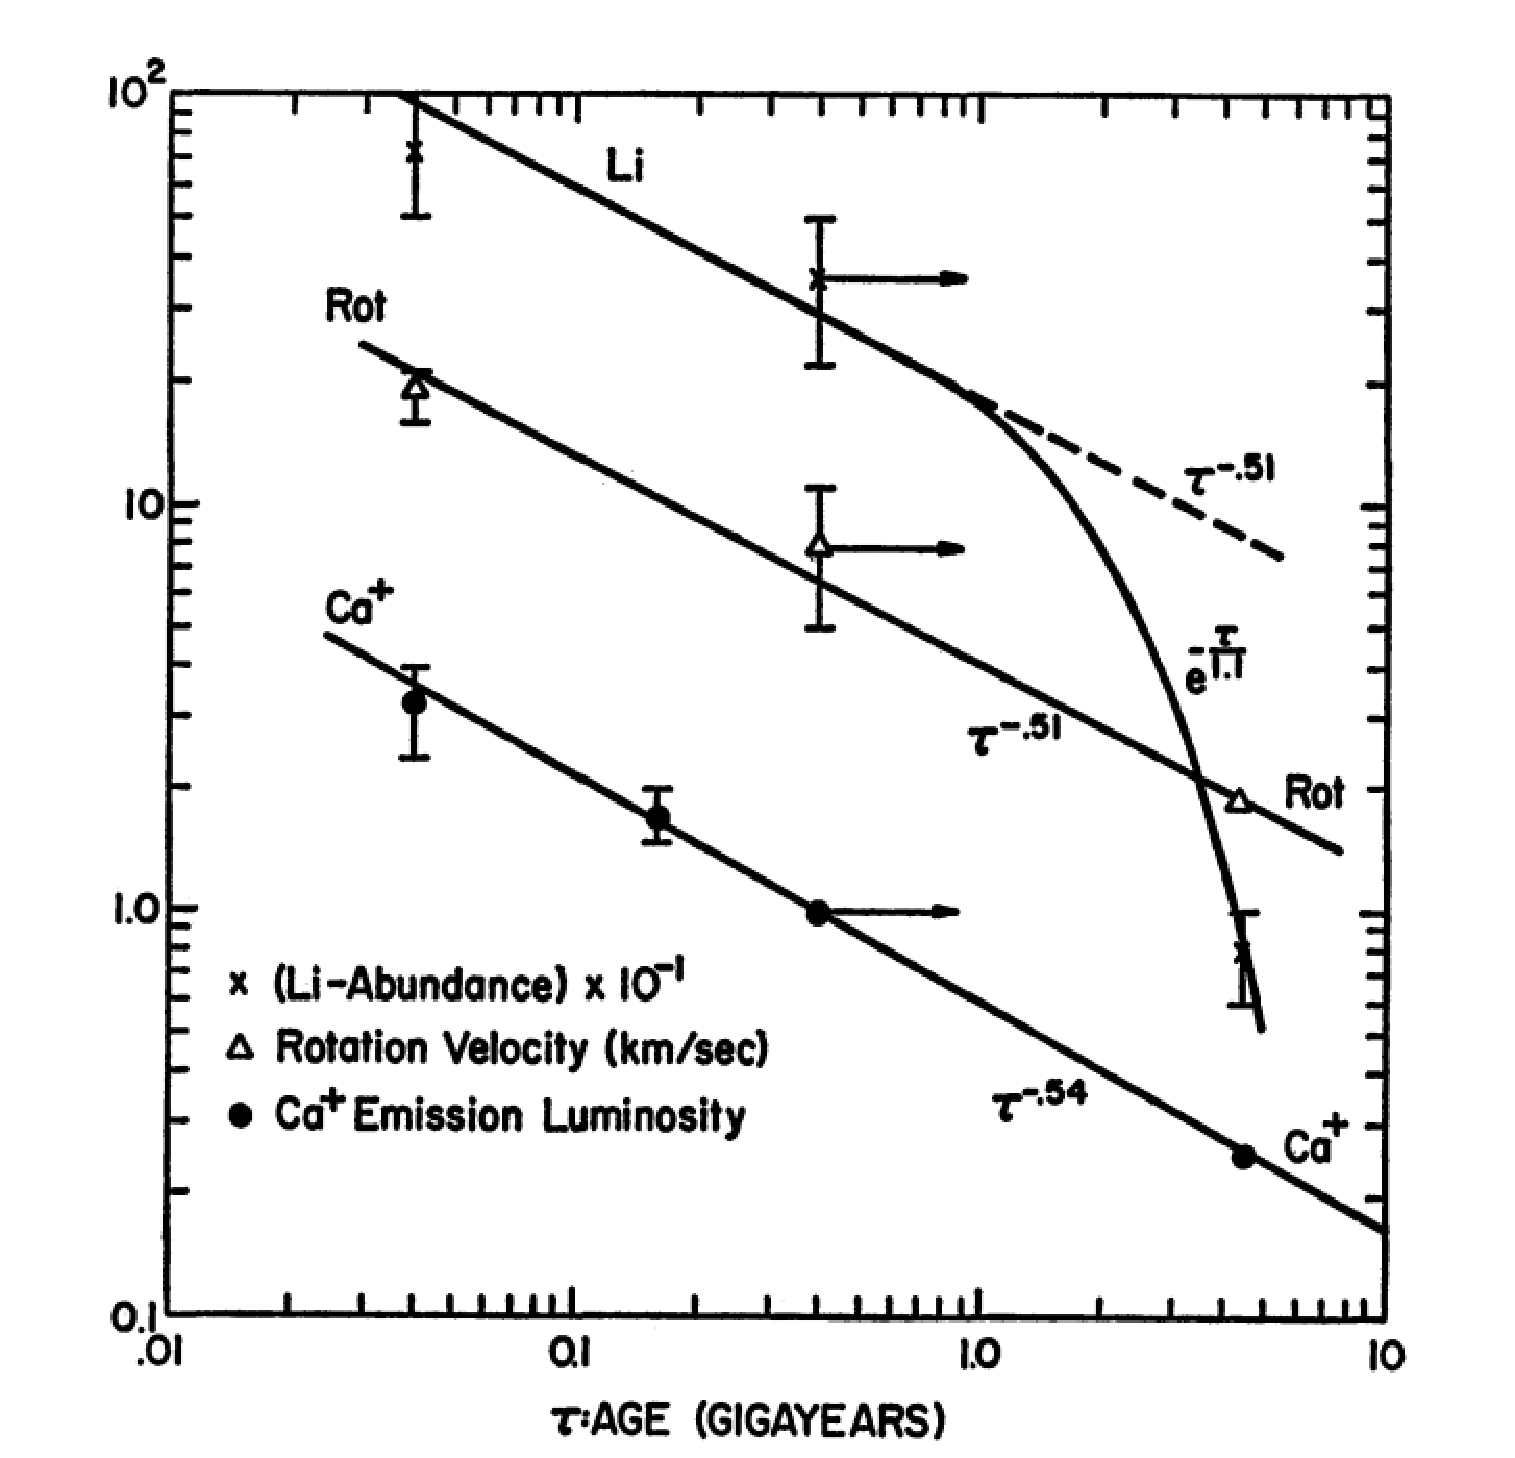
\includegraphics[width=6in, clip=true]{figures/skumanich.pdf}
\caption{Figure from \citet{skumanich1972}. Rotation periods for the G stars
in the Hyades and Pleiades and the Sun are plotted.}
\label{fig:skumanich}
\end{center}
\end{figure}

% kraft

% kawaler
% barnes

\section{Other age diagnostics}

\subsection{Lithium depletion}
Lithium depletion is useful age diagnostic for young stars.

\subsection{Proper motion}

\section{Stellar rotation}

\section{Statistics and hierarchical Bayes}
